\subsection{Regression Analysis}
\subsubsection{Plain and Stochastic Gradient Descent}
\begin{figure}[ht!]
    \centering
    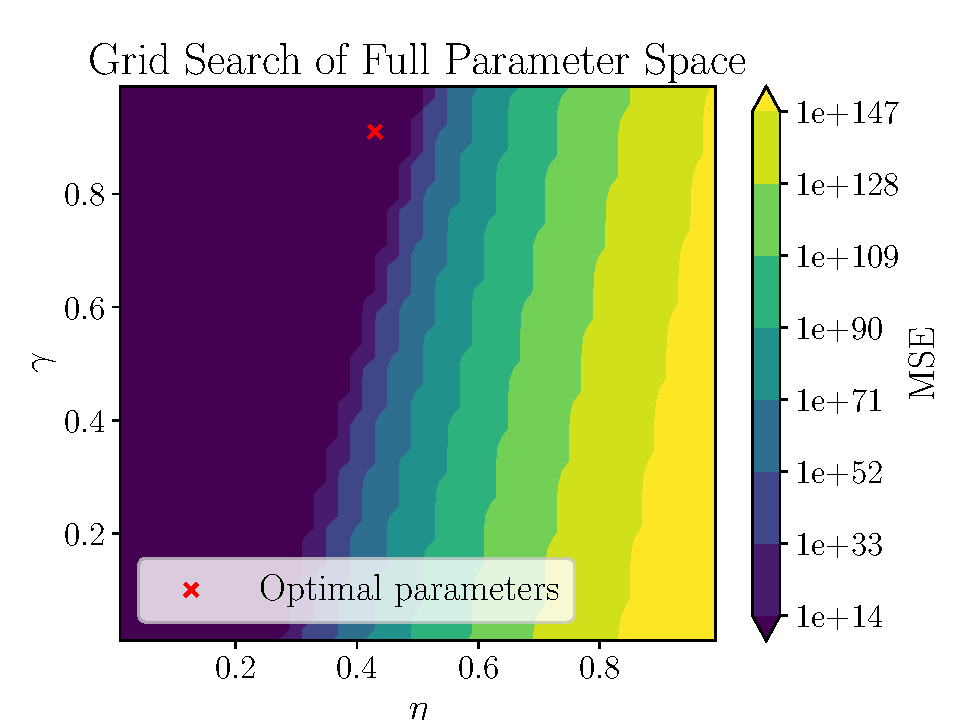
\includegraphics[width = .475\textwidth]{../figs/a_2_parameter_overview.pdf}
    \caption{Overview of the entire parameter space, plotting learning rate against momentum,  using plain gradient descent. The optimal parameters are marked with a red cross, to use as a starting point for further analysis.}
    \label{fig: param_overview}
\end{figure}
\begin{figure}[ht!]
    \centering
    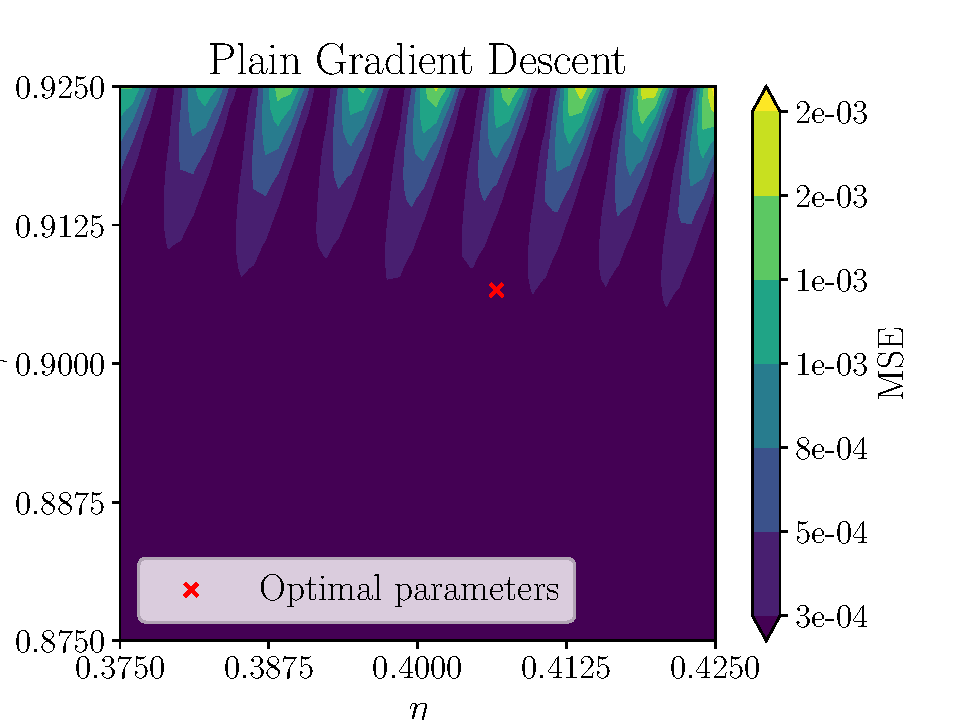
\includegraphics[width = .475\textwidth]{../figs/GD_eta_gamma.pdf}
    \caption{Narrowed down parameter space from \cref{fig: param_overview}.}
    \label{fig: param_narrowed}
\end{figure}
\begin{figure}[ht!]
    \centering
    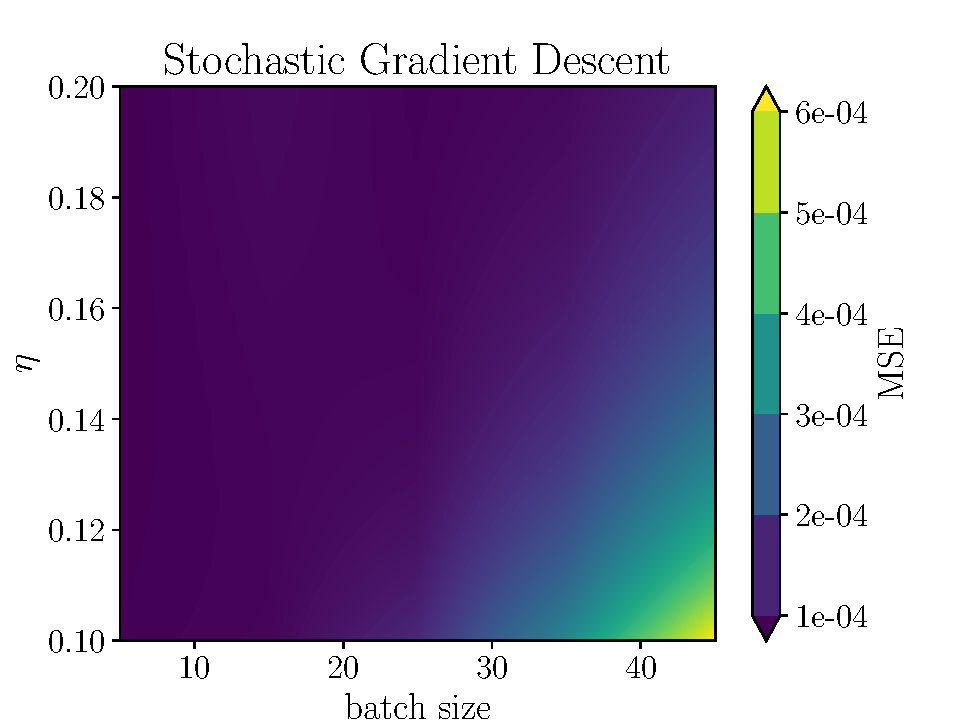
\includegraphics[width = .475\textwidth]{../figs/SGD_batch_eta_.pdf}
    \caption{Plotting batch size, against learning rate, using stochastic gradient descent.}
    \label{fig: SGD_batch_eta}
\end{figure}
\begin{figure}[ht!]
    \centering
    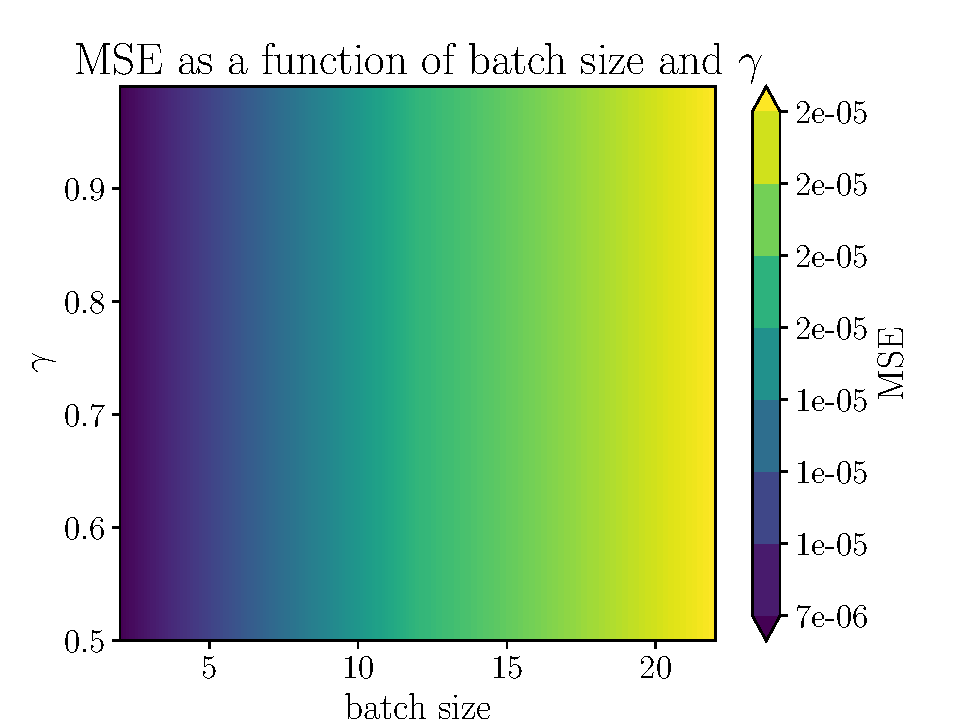
\includegraphics[width = 0.47575\textwidth]{../figs/SGD_batch_gamma.pdf}
    \caption{Plotting the batch size against the momentum, using stochastic gradient descent. Using a learning rate of $0.2$}
    \label{fig: SGD_batch_gamma}
\end{figure}

Looking at \cref{fig: param_overview} we found a region of parameters  in the upper-half , which gave the lowers MSE values. Using the best parameters found marked with a cross as a starting point, we found a good interval of values as seen in \cref{fig: param_narrowed}, with an order of magnitude around $10^{-4}$ and $10^{-3}$. In the following results, we only present the best intervals.

Continuing our search for the optimal batch number, we found between 5 and 20 batches to work well. In \cref{fig: SGD_batch_eta} without momentum. As a learning of $0.2$ gave the best results, we used this as our fixed learning rate in \cref{fig: SGD_batch_gamma} to find an optimal number of batches as a function of momentum. We see that the effect of changing the momentum is almost negligible, and that the number of batches is the most important parameter to tune. Even though we see a clear gradient in the plot, we find a large area with MSE values in the order of magnitude of \(10^{-5}\). The same is true in \cref{fig: SGD_batch_eta}, where over half of the learning rates between $0.1$ and $0.2$ give MSE values around \(10^{-4}\).

\subsubsection{AdaGrad}
\begin{figure}[ht!]
    \centering
    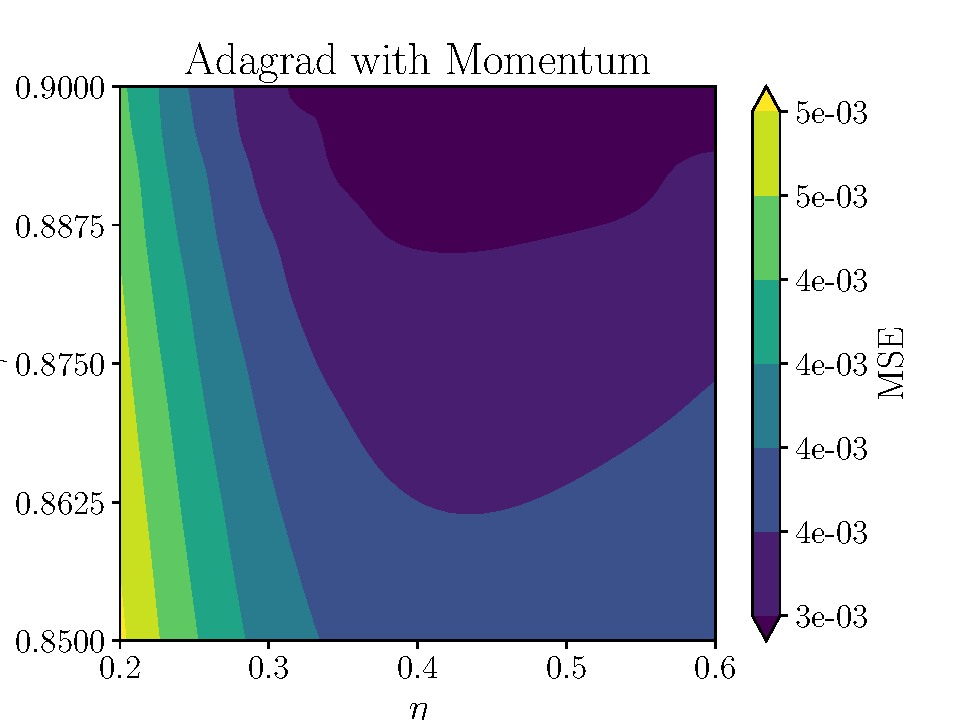
\includegraphics[width = 0.475\textwidth]{../figs/AdagradMomentum_eta_gamma.pdf}
    \caption{Plotting the learning rate against the momentum, using regular AdaGrad}
    \label{fig: AdagradMomentum_eta_gamma}
\end{figure}
\begin{figure}[ht!]
    \centering
    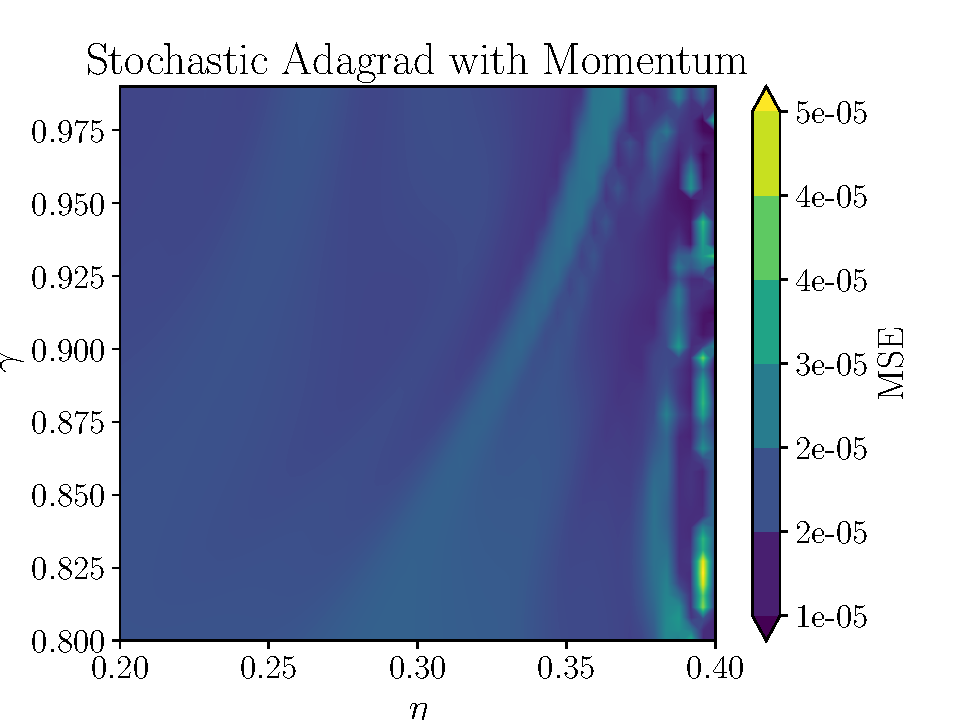
\includegraphics[width = 0.475\textwidth]{../figs/AdagradMomentum_stochastic_eta_gamma.pdf}
    \caption{Plotting the learning rate against the momentum, using stochastic AdaGrad. The batch size is set to 20.}
    \label{fig: AdagradMomentum_stochastic_eta_gamma}
\end{figure}
Exploring further with \cref{fig: AdagradMomentum_eta_gamma} and \cref{fig: AdagradMomentum_stochastic_eta_gamma} we found that the stochastic performed better then plain gradient descent, of 2 orders of magnitude. The stochastic version had an MSE of around \(10^{-5}\), while the plain version had an MSE of around \(10^{-3}\).

\subsubsection{RMSprop}
\begin{figure}[ht!]
    \centering
    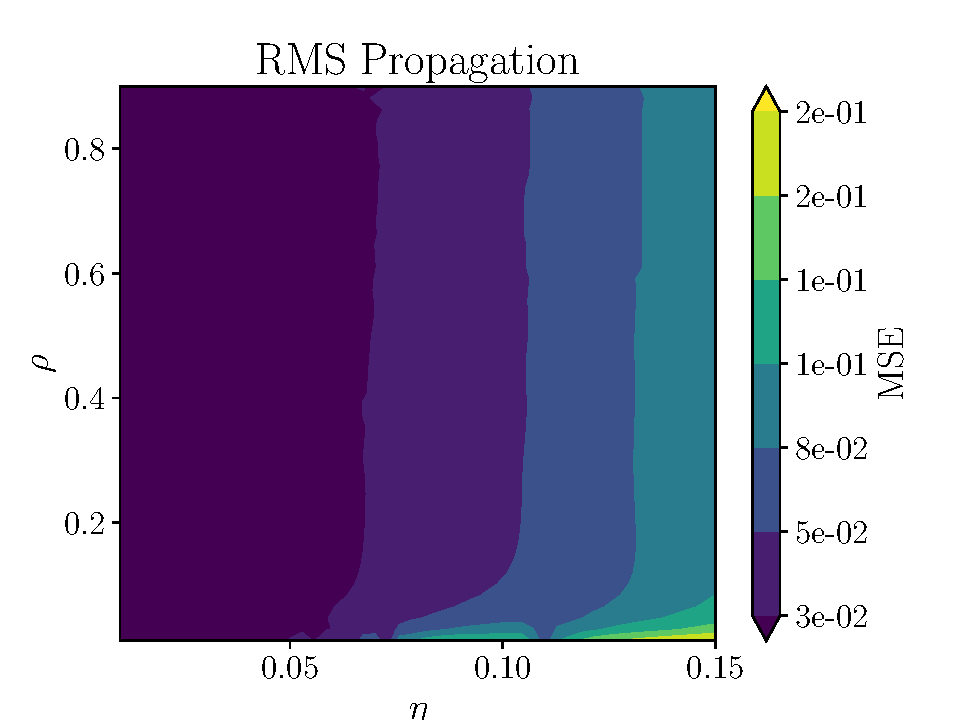
\includegraphics[width = 0.475\textwidth]{../figs/RMS_Prop_eta_rho.pdf}
    \caption{Plotting the learning rate against the decay rate, using RMSprop}
    \label{fig: RMS_Prop_eta_rho}
\end{figure}

\begin{figure}[ht!]
    \centering
    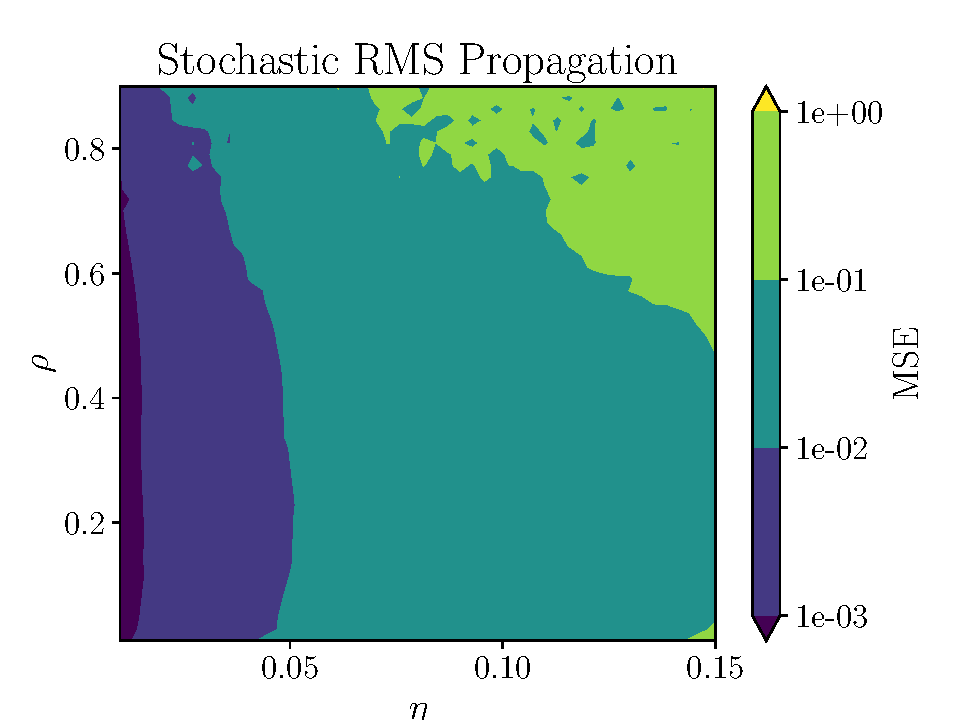
\includegraphics[width = 0.475\textwidth]{../figs/RMS_Prop_stochastic_eta_rho.pdf}
    \caption{Plotting the learning rate against the decay rate, using stochastic RMSprop. The batch size is set to 20.}
    \label{fig: RMS_Prop_stochastic_eta_rho}
\end{figure}
The RMS propagation method was very sensitive to the learning rate. As seen in \cref{fig: RMS_Prop_eta_rho} and \cref{fig: RMS_Prop_stochastic_eta_rho}, there was only a narrow range of learning rates that gave good results. Outside of this range, computation became unstable, and a lot of NaN values were produced. The stochastic version performed better than the plain version, with an MSE of around \(10^{-3}\) compared to \(10^{-2}\). Looking closer at the MSE values of the stochastic variant, we found some spots with MSEs with a value around \( 10^{-4} \). For the plain version, we found some spots with an MSE of around \( 10^{-3} \).

\subsubsection{Adam}
\begin{figure}[ht!]
    \centering
    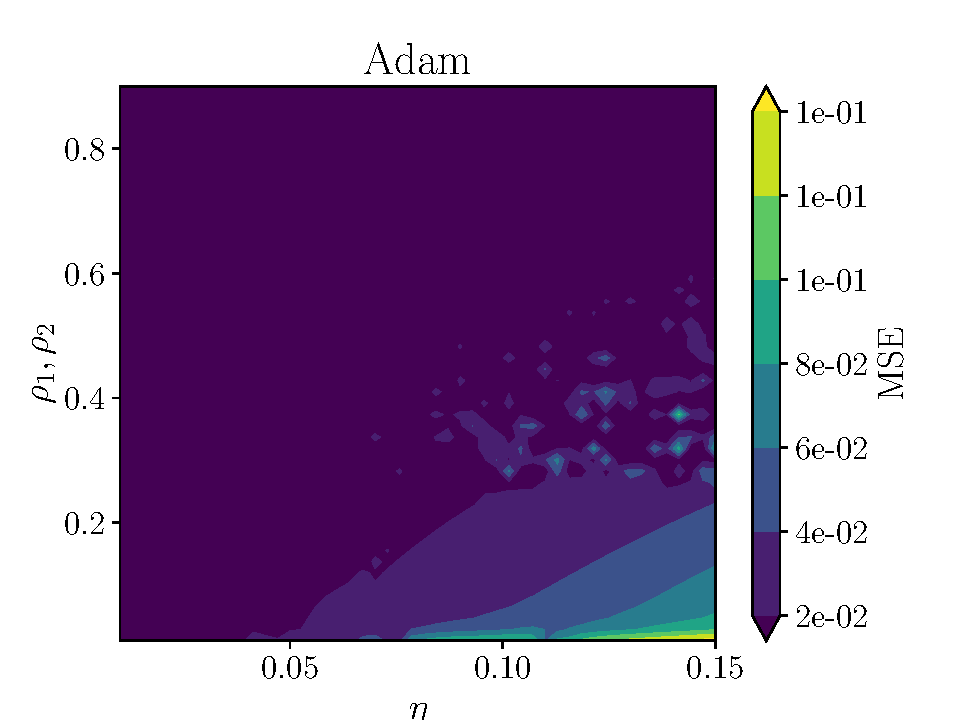
\includegraphics[width = 0.475\textwidth]{../figs/Adam_eta_rho.pdf}
    \caption{Plotting the learning rate against the decay rate. We have set the same value for $\rho_1$ and $\rho_2$, using Adam}
    \label{fig: Adam_eta_rho.pdf}
\end{figure}
\begin{figure}[ht!]
    \centering
    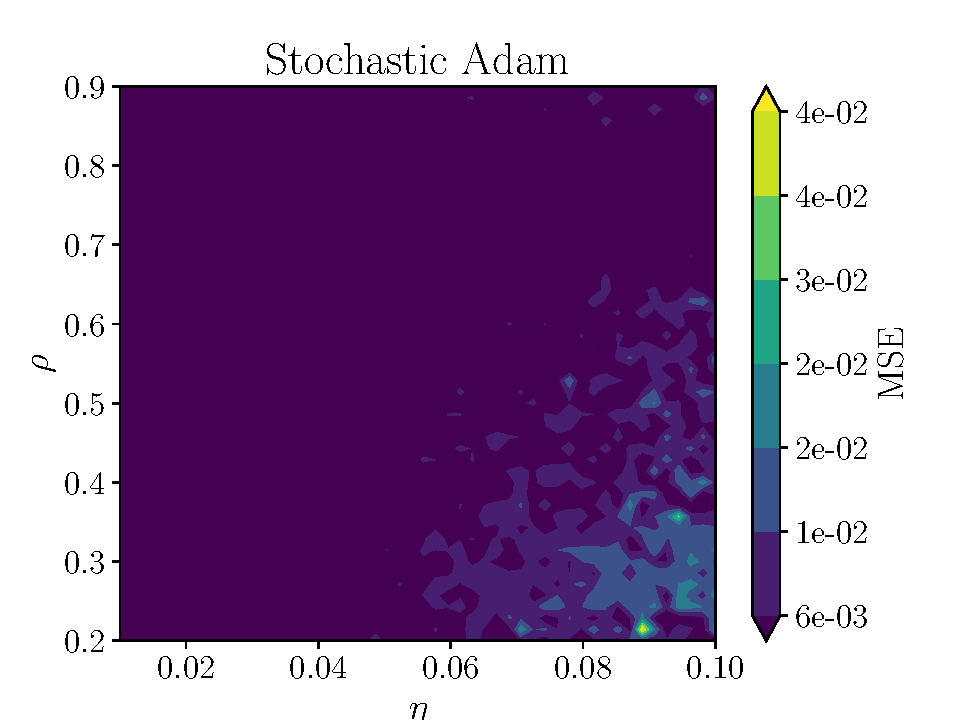
\includegraphics[width = 0.475\textwidth]{../figs/Adam_stochastic_eta_rho.pdf}
    \caption{Plotting the learning rate against the decay rate, using stochastic Adam. The batch size is set to 20, and the same value for $\rho_1$ and $\rho_2$ is used.}
    \label{fig: Adam_stochastic_eta_rho.pdf}
\end{figure}

The Adam optimization method was both unstable and very sensitive to the learning rate. As seen in \cref{fig: Adam_eta_rho.pdf} and \cref{fig: Adam_stochastic_eta_rho.pdf}, the plain version had at best an MSE of around \(10^{-2}\), while the stochastic version had an MSE of around \(10^{-3}\). The stochastic version had some spots with an MSE of around \(10^{-6}\). The plain version had some spots with an MSE of around \(10^{-4}\).

\subsection{Neural Networks Regression}

Our analysis of feed-forward neural networks began with the Franke function regression problem, allowing us to validate our implementation and explore the effects of various hyperparameters. The results demonstrate that our neural network implementation achieves robust performance across a wide range of configurations, with optimal models achieving MSE values around \( 10^{-3} \) and \( R^2 \) scores above 0.95.

\onecolumngrid
\begin{figure}[ht!]
    \centering
    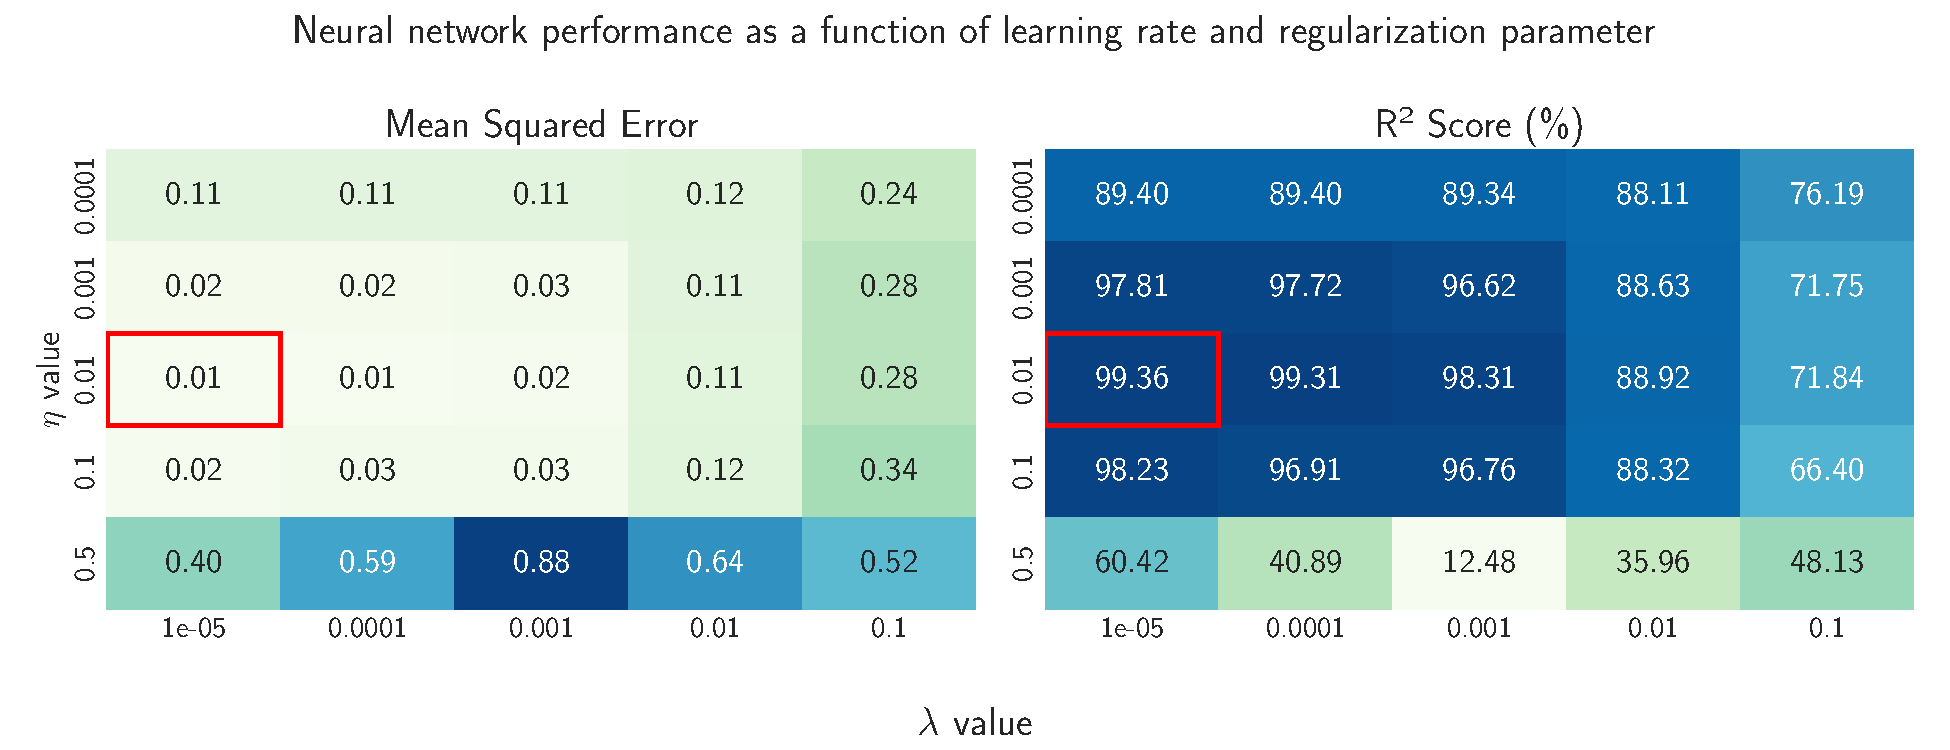
\includegraphics[width = .9\textwidth]{../figs/c_eta_lambda.pdf}
    \caption{The effect of learning rate and regularization strength on the Franke function regression problem. The plot shows the MSE and \( R^2 \) scores for different combinations of learning rate and regularization strength, with the optimal values highlighted in red.}
    \label{fig:NN_Franke_eta_lambda}
\end{figure}
\twocolumngrid

Our feed-forward neural network demonstrated consistently strong performance on the Franke function regression task across a range of hyperparameters. As shown in \cref{fig:NN_Franke_eta_lambda}, the model achieves stable MSE scores around $10^{-3}$ and $R^2$ scores above 0.99 for combinations of learning rates $ \eta $ in the range $ 10^{-1} $ to $ 10^{-3}$ and regularization strengths $ \lambda $ in $ 10^{-3} $ to $ 10^{-5}$ . The model only shows significant performance degradation with the highest tested learning rate ($\eta = 0.5$), suggesting robust behavior across most of the hyperparameter space.

\onecolumngrid
\begin{figure}[ht!]
    \centering
    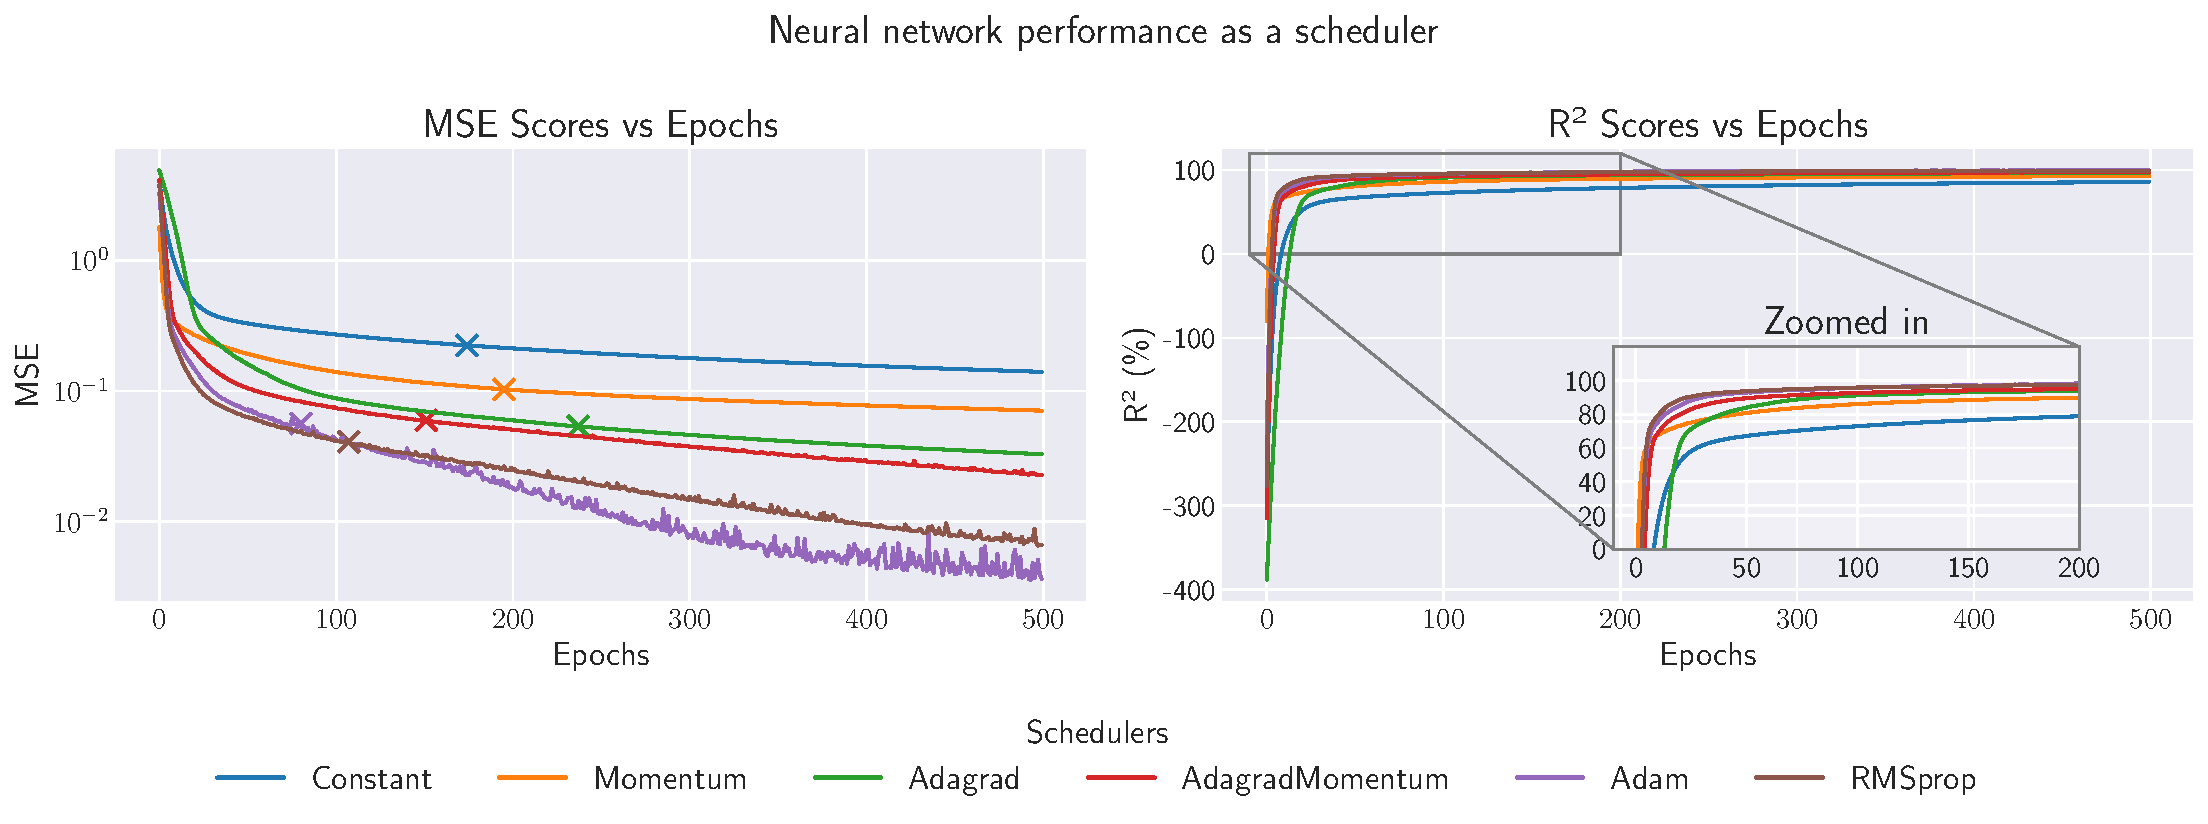
\includegraphics[width = .9\textwidth]{../figs/b_schedulers.pdf}
    \caption{The effect of different learning rate schedulers on the Franke function regression problem. The plot shows the training MSE and \( R^2 \) scores for different learning rate schedulers as a function of epochs. The schedulers MSEs are marked with a cross indicating at which epoch convergence was reached.}
    \label{fig:NN_Franke_schedulers}
\end{figure}
\twocolumngrid

The comparison of different optimization schedulers in \cref{fig:NN_Franke_schedulers} shows that all implemented methods have varying success with Adam and RMSprop performing the best. The marked convergence points indicate that both Adagrad methods are slower to converge than the other methods, while RMSprop reach its point around just 100 epochs. As the criteria for convergence is chosen somewhat arbitrarily, as describe in \cref{subsec:nn_schedulers}, the marked crosses may not showcase where the schedulers converge, but gives insight into when the learning rates are slowing down relative to eachother as the networks are training. The figure also suggest that given enough epochs, both Adagrads, Adam and RMSprop will converge to an mse of just short of \( 10^{-3} \) and an \( R^2 \) score of 0.95. While constant learning rate and plain momentum will perform worse.

\onecolumngrid
\begin{figure}[ht!]
    \centering
    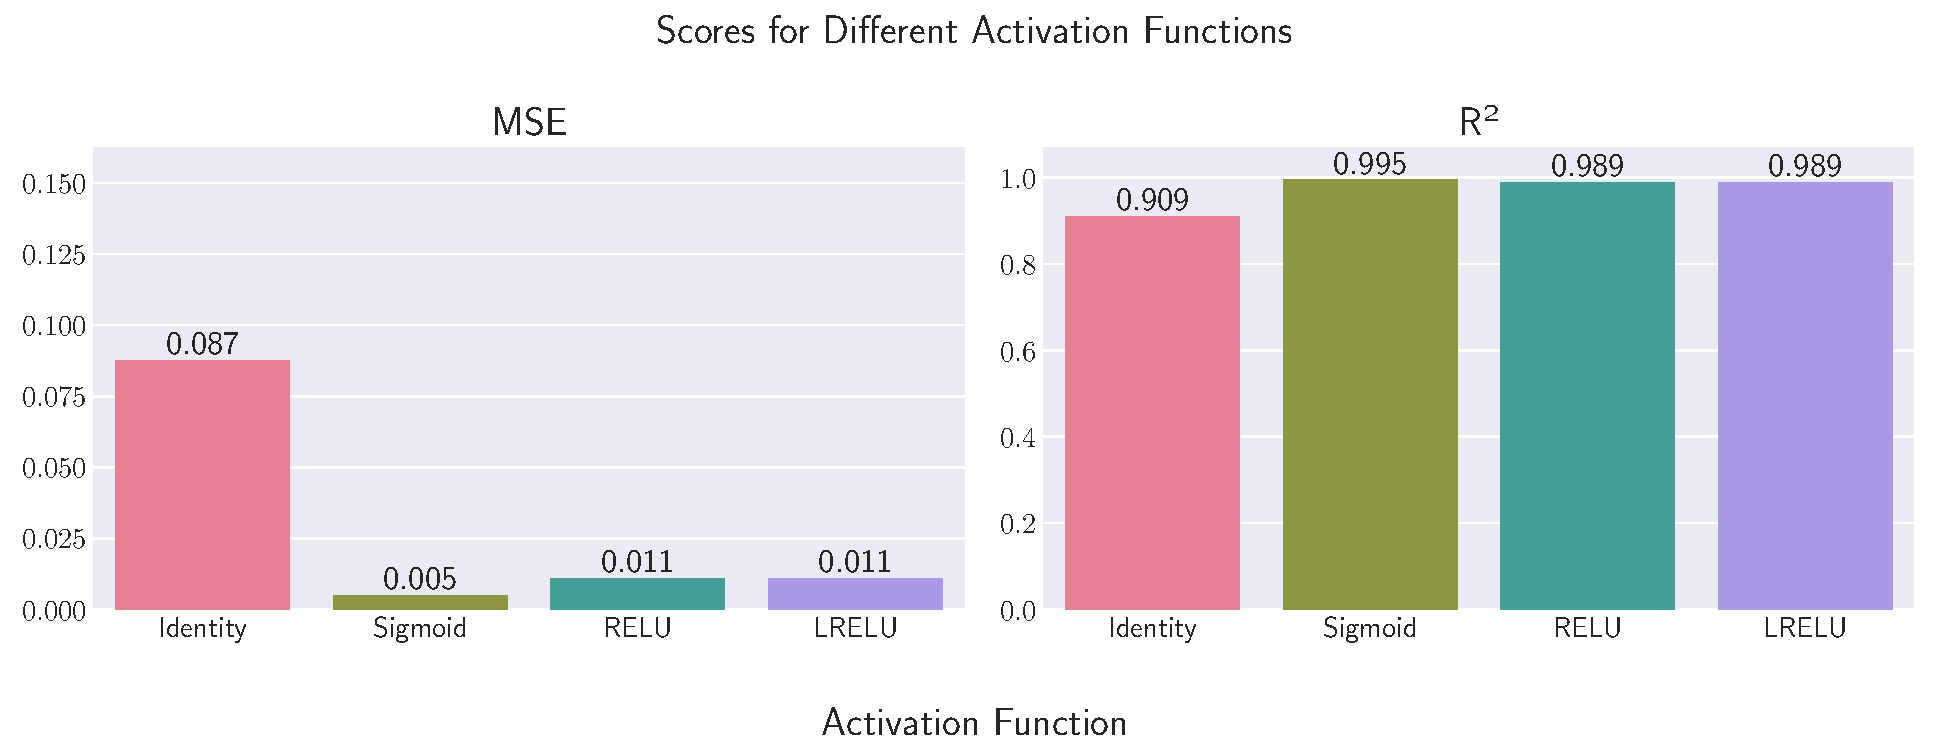
\includegraphics[width = .9\textwidth]{../figs/c_activation_funcs.pdf}
    \caption{The effect of different activation functions on the Franke function regression problem. The plot shows the test MSE and \( R^2 \) scores for different activation functions.}
    \label{fig:NN_Franke_activation}
\end{figure}
\twocolumngrid

Testing different activation functions (\cref{fig:NN_Franke_activation}), reveals similar performance levels among non-linear functions. The sigmoid activation in the hidden layer performs slightly better with an MSE of $0.005$ and $R^2$ of $0.995$, but ReLU and Leaky ReLU follow closely with MSE around $0.011$ and $R^2$ of $0.989$. As expected, removing the non-linear capability of the network by using the identity function in the hidden layer results in significantly worse performance, with an MSE of $\approx 0.09$ and $R^2$ of $\approx0.91$.

\onecolumngrid
\begin{figure}[ht!]
    \centering
    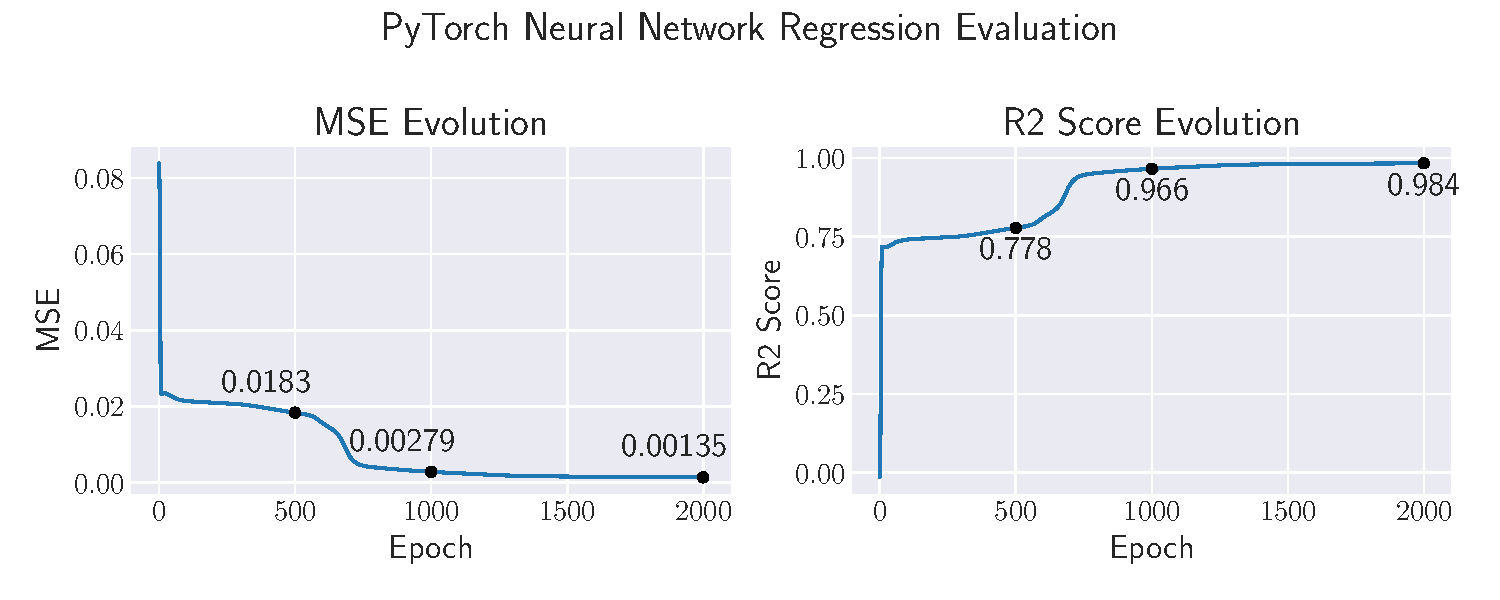
\includegraphics[width = .9\textwidth]{../figs/nn_torch_franke.pdf}
    \caption{PyTorch neural network regression on the Franke function. The plot shows the training and test MSE and \( R^2 \) as a function of epochs. The plots are annotated with the values at epochs 500, 1000 and 2000}
    \label{fig:NN_Torch_scores}
\end{figure}
\twocolumngrid

Comparing our results with the PyTorch implementation in \cref{fig:NN_Torch_scores}, we see that our model performed similarly to the PyTorch model, with an MSE around \( 10^{-3} \) and an \( R^2 \) score around 0.95. The main takeaway from this is that our models were faster to reach stable performance, wile the PyTorch model took more epochs to become stable at slightly better performance. This might suggest that the PyTorch model is more robust to overfitting, but at the cost of longer training times.

\clearpage

\subsection{Neural Networks Classification}

\onecolumngrid
\begin{figure}[ht!]
    \centering
    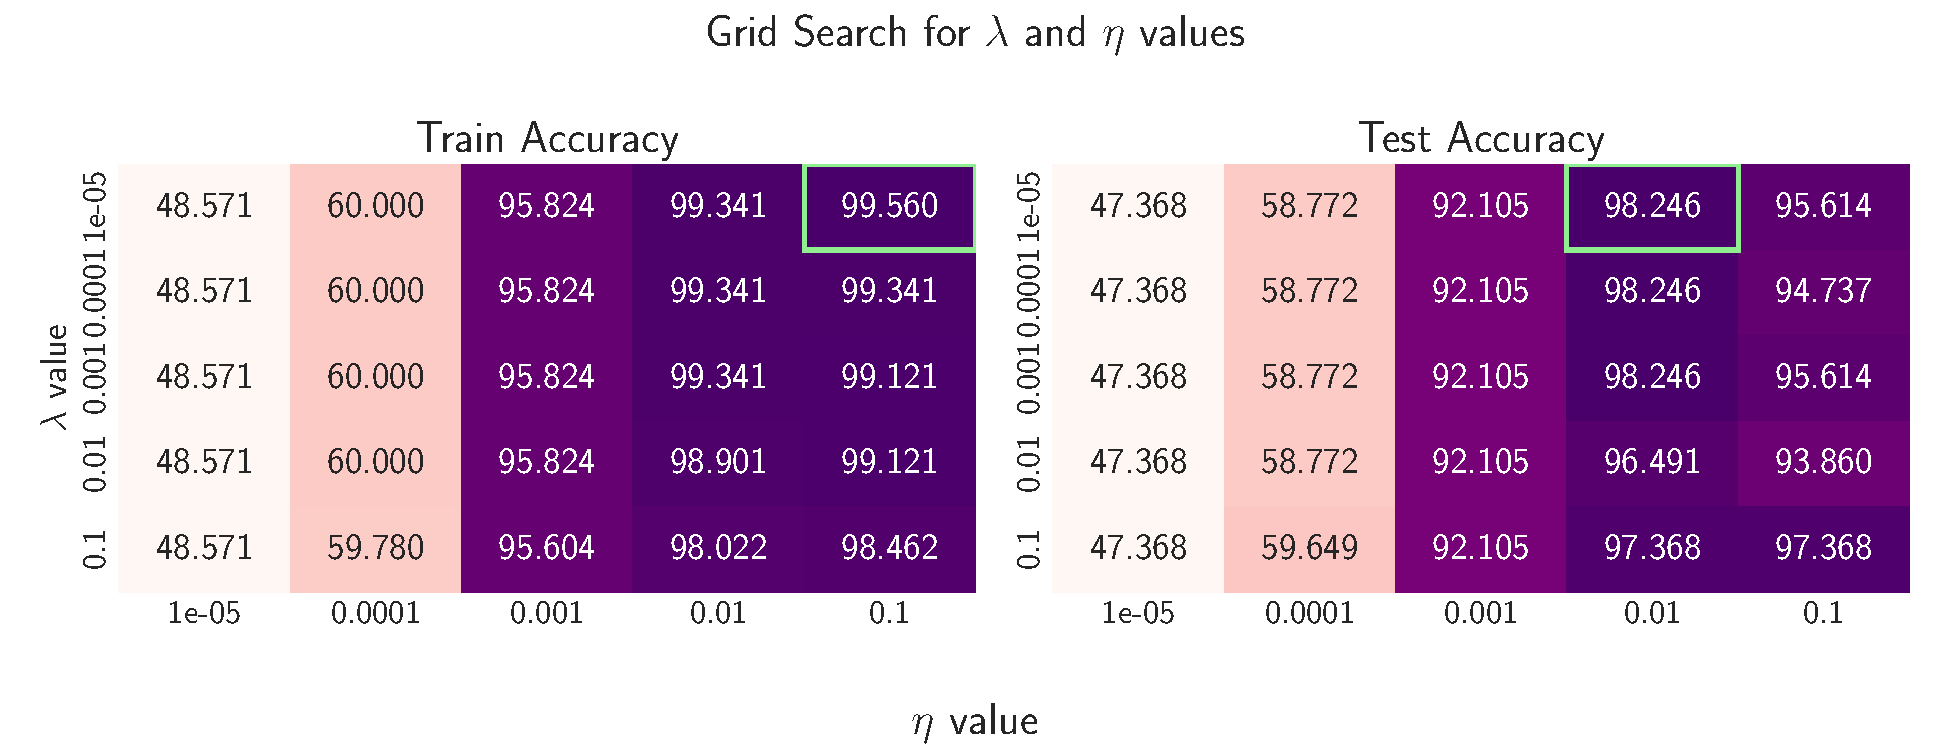
\includegraphics[width = .9\textwidth]{../figs/classification_lambda_eta.pdf}
    \caption{Model performance for different learning rates and regularization strengths on the breast cancer classification problem. The plot shows the training and test accuracy scores for different combinations of learning rate and regularization strength. The optimal values are highlighted in green.}
    \label{fig:NN_Classification_lambda_eta}
\end{figure}
\twocolumngrid

Our feed-forward neural network achieved strong classification performance on the Wisconsin Breast Cancer dataset. As shown in \cref{fig:NN_Classification_lambda_eta}, the model maintains high accuracy ($<95\%$) across a broad range of hyperparameter combinations. Performance is most dependent on the learning rate, having optimal performance for $\eta$ between $10^{-1}$ and $10^{-2}$, while the regularization strength is less critical with a slight trend for better performance with lower $\lambda$ values. In the figure, the optimal values for training accuracy and test accuracy differ. Since the dataset is small, the model is prone to overfitting and this could be the reason for the discrepancy.

\onecolumngrid
\begin{figure}[ht!]
    \centering
    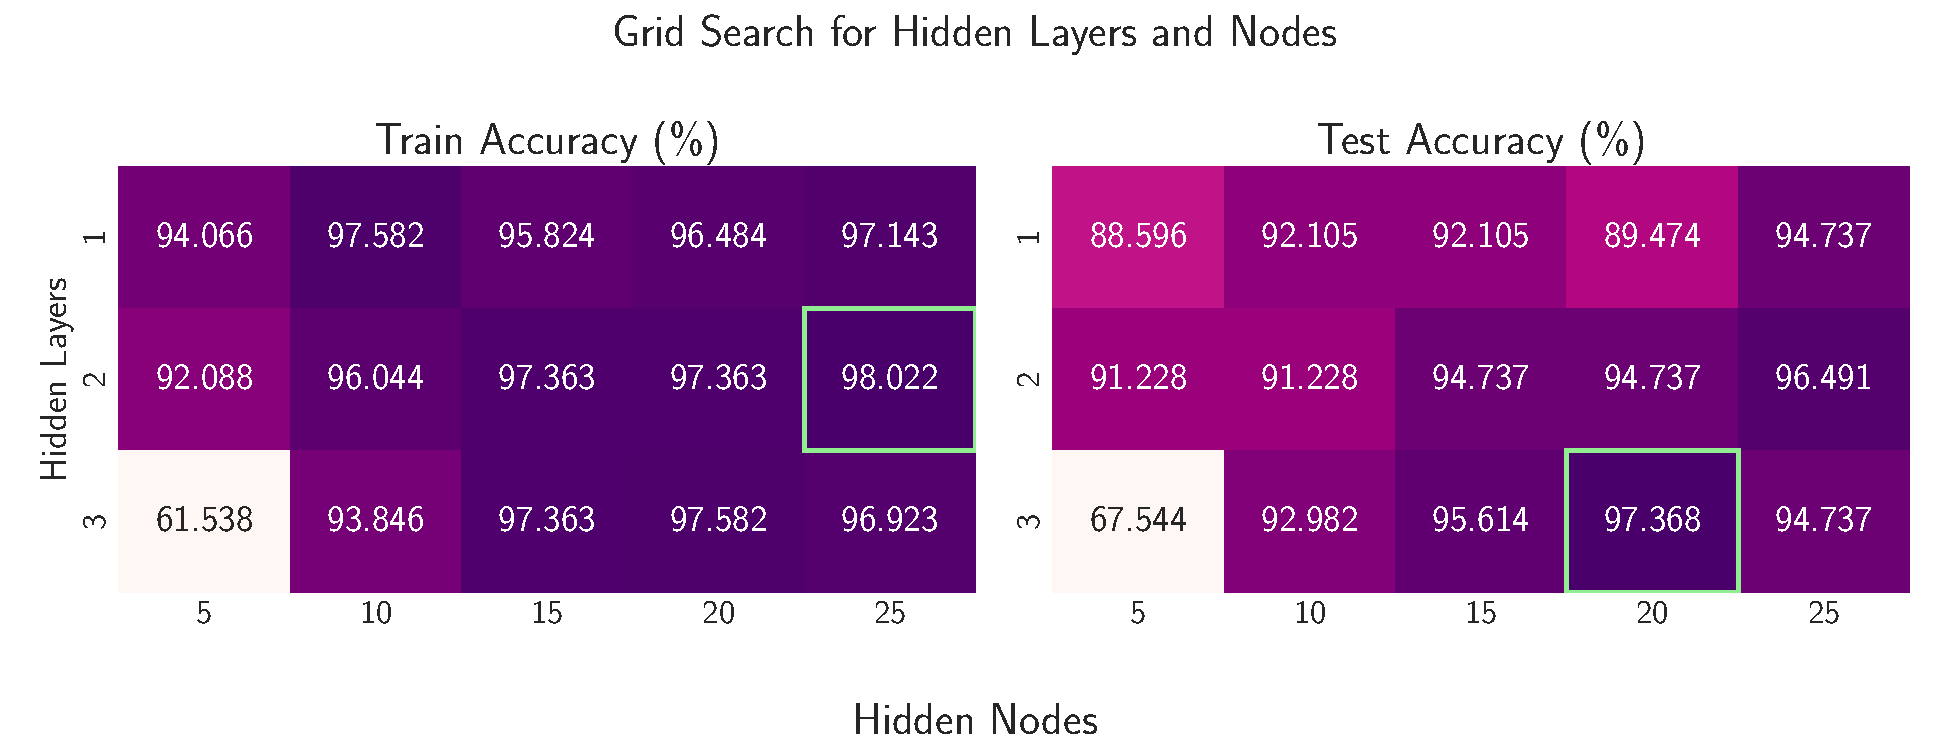
\includegraphics[width = .9\textwidth]{../figs/classification_hidden_layers_nodes.pdf}
    \caption{Model performance for different network architectures on the breast cancer classification problem. The plot shows the training and test accuracy scores for different numbers of hidden layers and nodes. The optimal values are highlighted in green.}
    \label{fig:NN_Classification_hidden_layers_nodes}
\end{figure}
\twocolumngrid

The exploration of network architectures demonstrates that model performance remains robust across different configurations. Networks with 2-3 hidden layers and 15-25 nodes per layer consistently achieve test accuracies above 96\%. Notably, very small networks (5 nodes) show degraded performance, particularly with three layers where training accuracy drops to 61.5\%, suggesting insufficient model capacity. Our initial assumptions that it would suffice to have a small network for this dataset are somewhat backed up by the results, but the faster runtimes do have a tradeoff in performance.

\onecolumngrid
\begin{figure}[ht!]
    \centering
    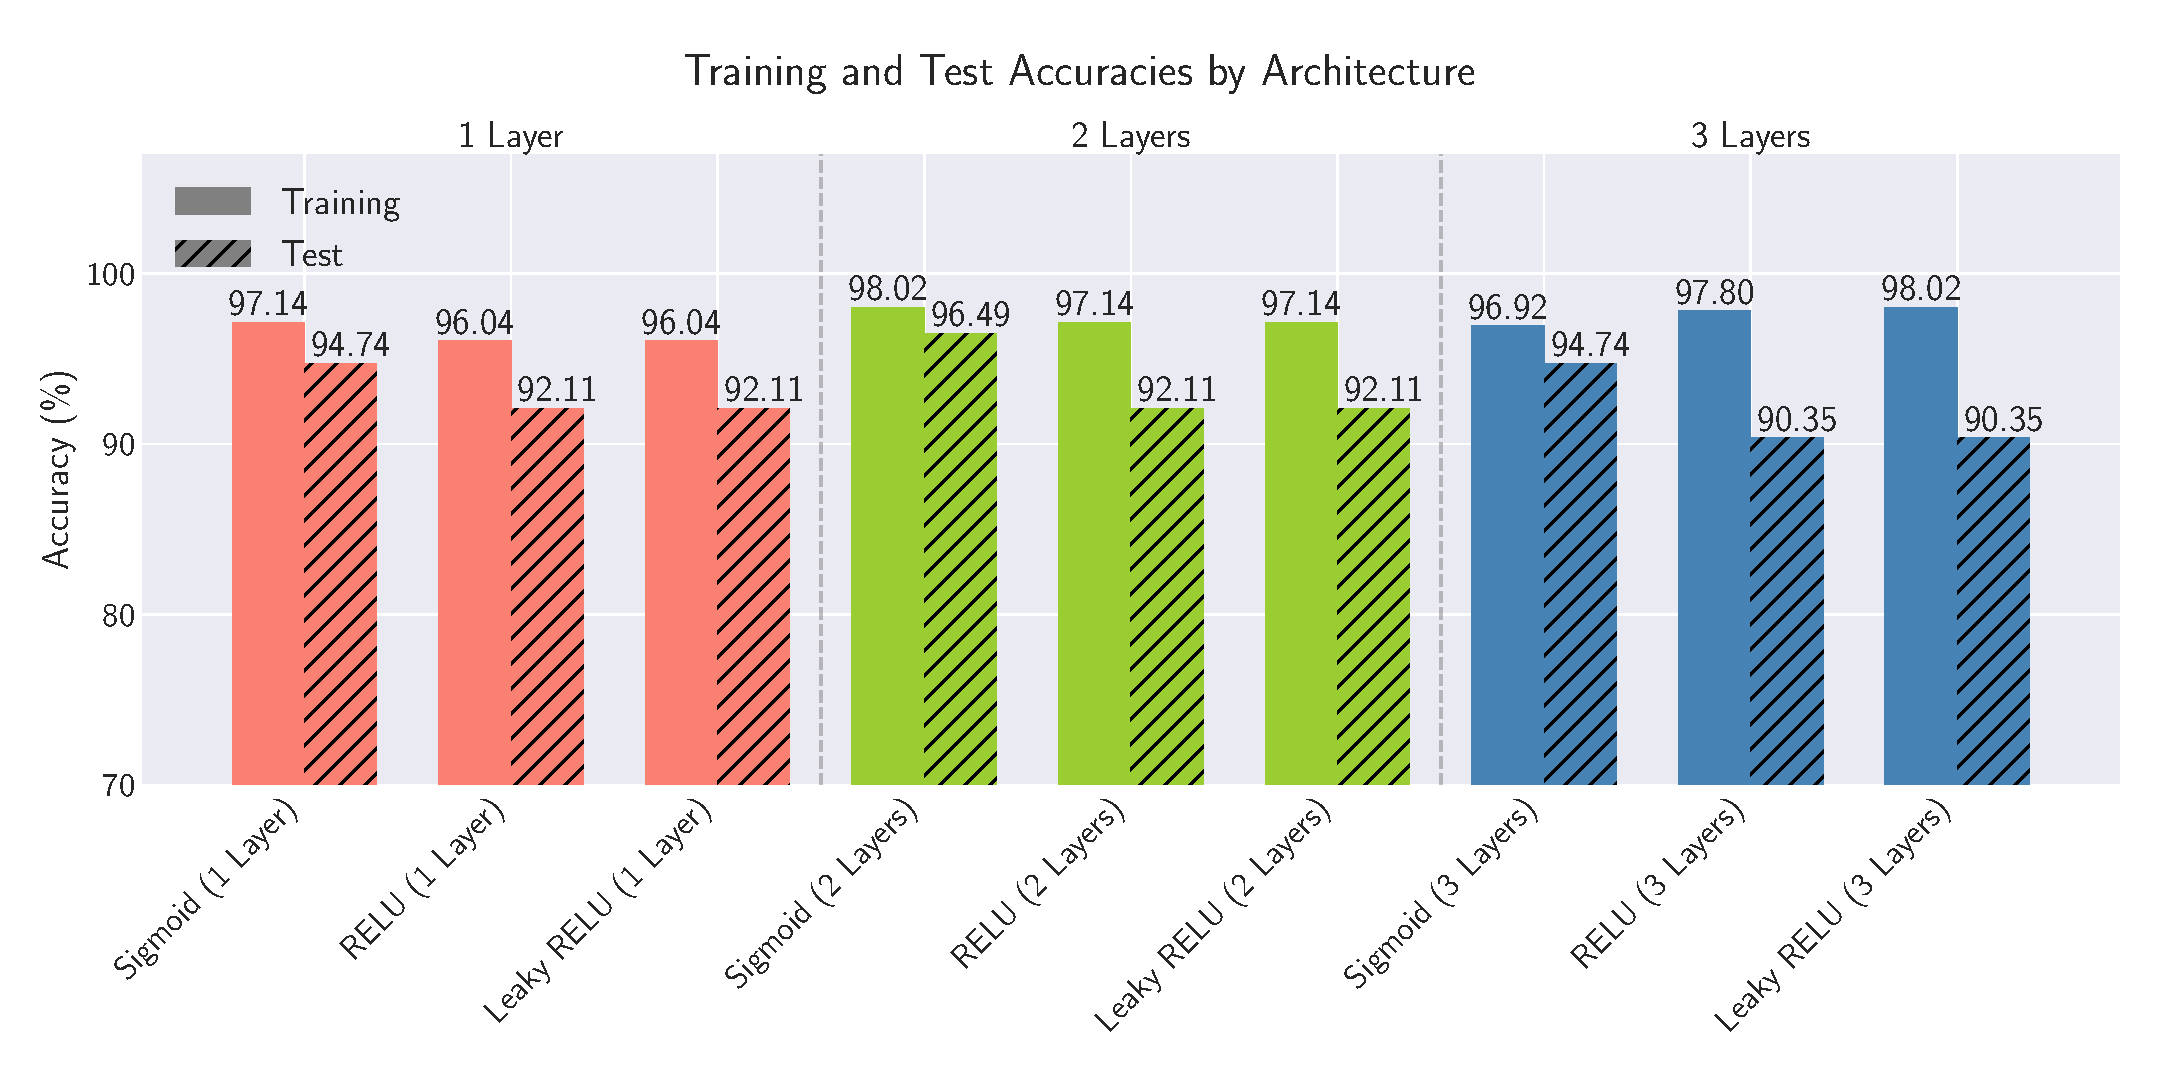
\includegraphics[width = .9\textwidth]{../figs/classification_activations_layers.pdf}
    \caption{Model performance for different activation functions on the breast cancer classification problem. The plot shows the training and test accuracy scores for different activation functions and numbers of hidden layers.}
    \label{fig:NN_Classification_activations_layers}
\end{figure}
\twocolumngrid

All tested activation functions perform similarly well, with accuracy variations within 2-3 percentage points. In single-layer configurations, sigmoid achieves slightly better performance, while ReLU and Leaky ReLU trends to better performance in deeper networks. This is only true for the training data, as all test accuracies degrade with more layers. This again suggest the danger of overfitting, and that the dataset is too small to support deep networks.

\begin{figure}[ht!]
    \centering
    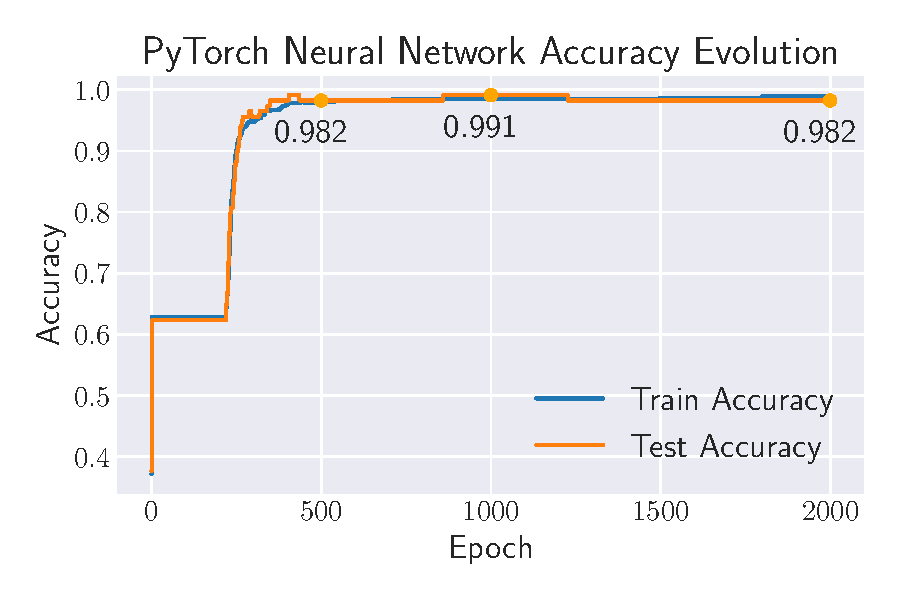
\includegraphics[width =.45\textwidth]{../figs/nn_torch_breast_cancer.pdf}
    \caption{PyTorch neural network classification on the breast cancer dataset. The plot shows the training and test accuracy as a function of epochs. The figure is annotated with the test accuracies at epochs 500, 1000 and 2000.}
    \label{fig:NN_Torch_breast_cancer}
\end{figure}

From \cref{fig:NN_Torch_breast_cancer}, we see that the PyTorch model is a more stable model, taking more time to reach high performance levels, but manages to hold a test accuracy of $<98\%$ after 500 epochs. As our models are often scoring above 98\% after only 20 epochs. A possible explanation for this is that the PyTorch model is a more advanced model, increasing the difficulty to train the network compared to our relatively simple model for a small data set as the Wisconsin Breast Cancer data.

\subsection{Logistic Regression}

\onecolumngrid
\begin{figure}[ht!]
    \centering
    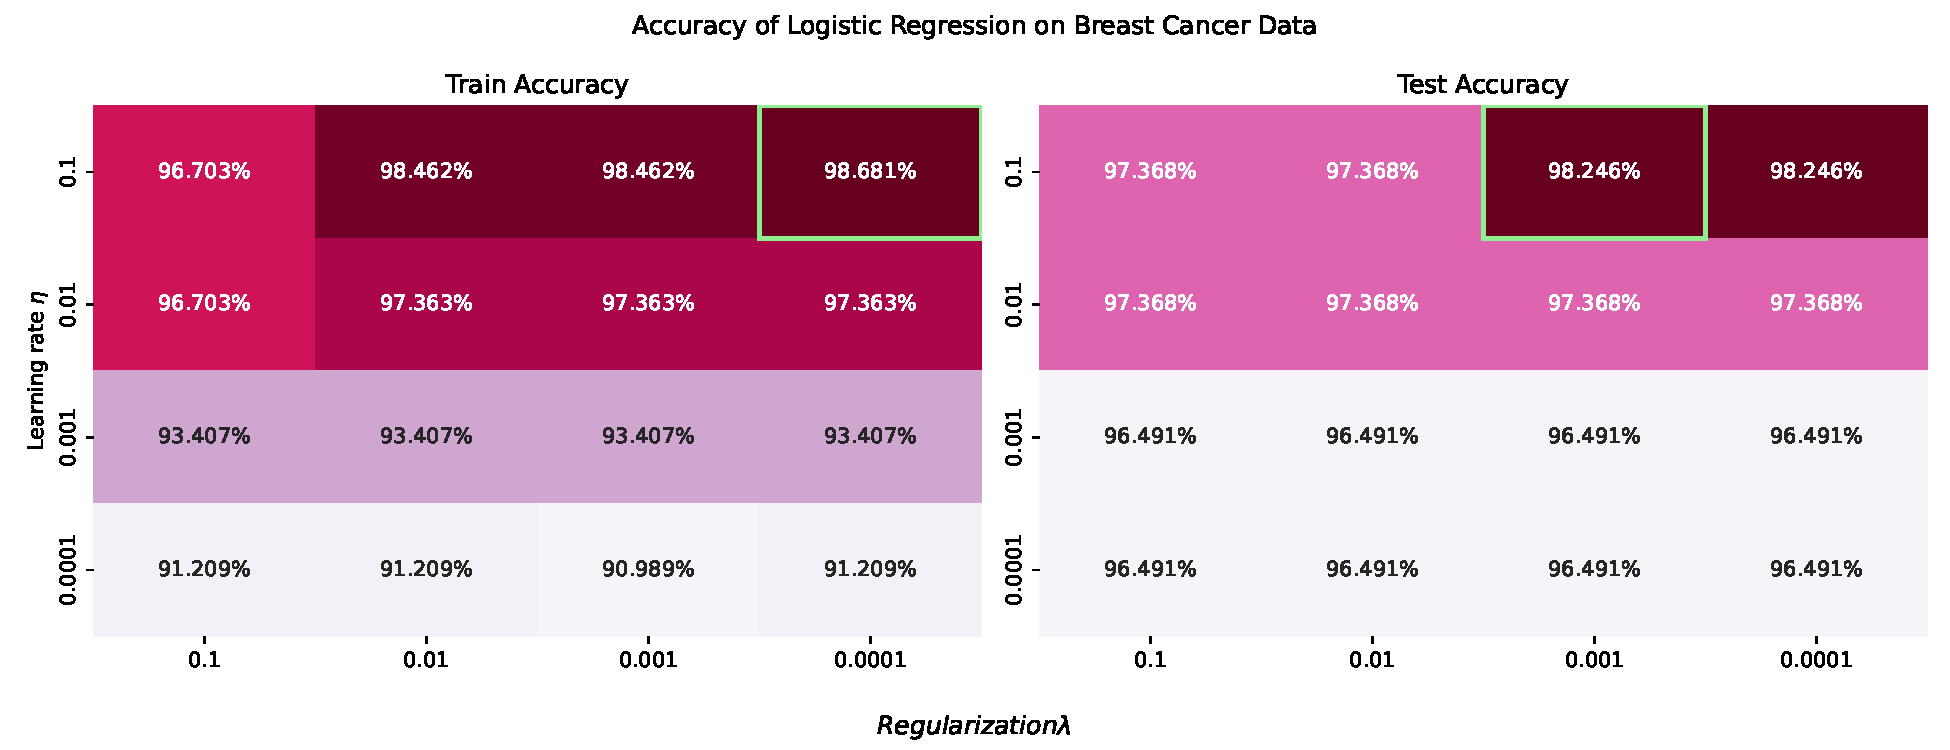
\includegraphics[width = .9\textwidth]{../figs/logistic_regression_gridsearch.pdf}
    \caption{Model performance for different learning rates and regularization strengths on the breast cancer classification problem using logistic regression. The plot shows the training and test accuracy scores for different combinations of learning rate and regularization strength. The optimal values are highlighted in green.}
    \label{fig:logistic_regression_gridsearch}
\end{figure}
\twocolumngrid

Our logistic regression implementation achieves high performance on the breast cancer dataset, with test accuracies consistently above 96\% across most hyperparameter combinations. \cref{fig:logistic_regression_gridsearch} shows that performance is robust across a wide range of learning rates and regularization strengths, with optimal test accuracy of 98.2\% achieved at $\eta$ = 0.0001 and a regularization strength of 0.1. The model demonstrates good generalization, with test accuracies closely matching training accuracies across the parameter space.

\begin{figure}[ht!]
    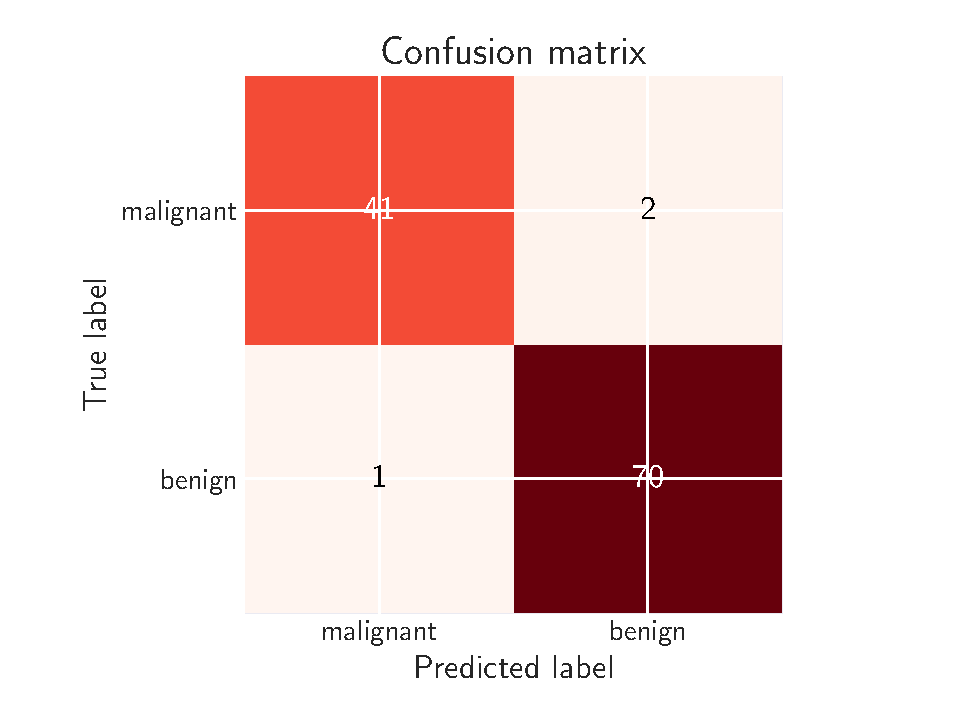
\includegraphics[width =.45\textwidth]{../figs/confusion_matrix.pdf}
    \caption{Confusion matrix for the breast cancer classification problem with Skikit's Logistic Regression. The plot shows the confusion matrix for the test set, with the number of true positives, true negatives, false positives, and false negatives.}
    \label{fig:confusion_matrix}
\end{figure}

The confusion matrix from scikit-learn's implementation (\cref{fig:confusion_matrix}) shows excellent classification performance with only 3 misclassified samples out of 114 test cases. The model correctly identified 41 out of 43 malignant cases and 70 out of 71 benign cases, demonstrating balanced performance across both classes. The similar performance between our implementation and scikit-learn's validates our approach while suggesting that the classification task may be well-suited for linear decision boundaries.

\clearpage

% \vspace*{-2.5pt}
